\section{Part A: Data Generation}
\begin{itemize}
    \item For each distribution, generate \textbf{replicates of data} with sizes $10$, $100$, and $1000$.  
    \item Each replicate should consist of $100$ samples.  
    \item Example: For ``10 replicates,'' generate 10 separate datasets, each with 100 samples.  
    \item For one replicate from each distribution, plot the distribution of the sample to ensure that it follows a uniform/power-law distribution.
\end{itemize}

\textbf{Implementation notes:}  
\begin{itemize}
    \item In \textbf{Python}, use \texttt{numpy.random.uniform} and \texttt{numpy.random.power}.%, and \texttt{numpy.random.pareto}.  
    \item In \textbf{R}, use \texttt{runif()}, \texttt{rplcon()} (for Power, with shape1 = $\alpha$, shape2 = 2.5).
        
\end{itemize}
-----\\

For each distribution, the replicates were generated according to the recommended NumPy functions, and in the case of the second distribution, I took the guidance of the Canvas announcement and used the Pareto distribution from numpy.random.pareto with alpha parameter set to 2.3. My implementation of the generation functions just wrap the corresponding NumPy calls that let me set the shape according to the replicate sizes. So for the replicate with size 10, I have a CSV with 10 columns, one for each set of 100 samples. These are the relevant utility functions:

\begin{verbatim}
def generate_uniform_replicates(low: float, high: float, sample_size: int, 
                                num_replicates: int) -> np.ndarray:
    """
    Generates the replicates of uniformly distributed data.
    
    :param low: Lower bound of uniform distribution
    :type low: float
    :param high: Upper bound of uniform distribution
    :type high: float
    :param sample_size: Number of samples per replicate
    :type sample_size: int
    :param num_replicates: Number of replicates to generate
    :type num_replicates: int
    :returns: Array containing the replicates.
    :rtype: np.ndarray
    """
    replicates = np.random.uniform(low=low, high=high, 
                                   size=(num_replicates, sample_size))
    return replicates

def generate_powerlaw_replicates(sample_size: int, 
                                 num_replicates: int) -> np.ndarray:
    """
    Generates the replicates of power-law distributed data using Pareto distribution.
    
    :param alpha: Shape parameter for the power-law distribution
    :type alpha: float
    :param sample_size: Number of samples per replicate
    :type sample_size: int
    :param num_replicates: Number of replicates to generate
    :type num_replicates: int
    :returns: Array containing the replicates.
    :rtype: np.ndarray
    """
    replicates = np.random.pareto(a=2.3, size=(num_replicates, sample_size))
    return replicates
\end{verbatim}

\begin{center}
\textbf{Figure 1:} Data generation functions for Uniform and Power-Law distributions.\\
\end{center}

To verify that the generated replicates follow their expected distributions, I plotted the distribution of a single replicate for both the distributions. The visualization function and corresponding plots are shown below:\\

\begin{verbatim}
def plot_single_replicate(data: np.ndarray, dist_name: str, 
                                       output_filename: str):
    """
    Plots the distribution of a single replicate.
    
    :param data: Single replicate samples
    :type data: np.ndarray
    :param dist_name: Name of the distribution
    :type dist_name: str
    :param output_filename: Filename for the figure
    :type output_filename: str
    """
    sns.set_style("whitegrid")
    sns.set_palette("muted")
    plt.figure(figsize=(10, 6))
    
    ax = sns.histplot(data, bins=50, stat='density', 
                     edgecolor='white', alpha=0.7)
    
    ax.set_xlabel('Value', fontsize=14, labelpad=15)
    ax.set_ylabel('Density', fontsize=14, labelpad=15)
    ax.set_title(f'Distribution of {dist_name} Replicate', 
                fontsize=16, pad=20)
    
    plt.tight_layout()
    plt.savefig(f"../figures/{output_filename}", bbox_inches='tight', dpi=300)
\end{verbatim}

\begin{center}
\textbf{Figure 2:} Visualization function for verifying the distribution shape.\\
\end{center}

\begin{center}
  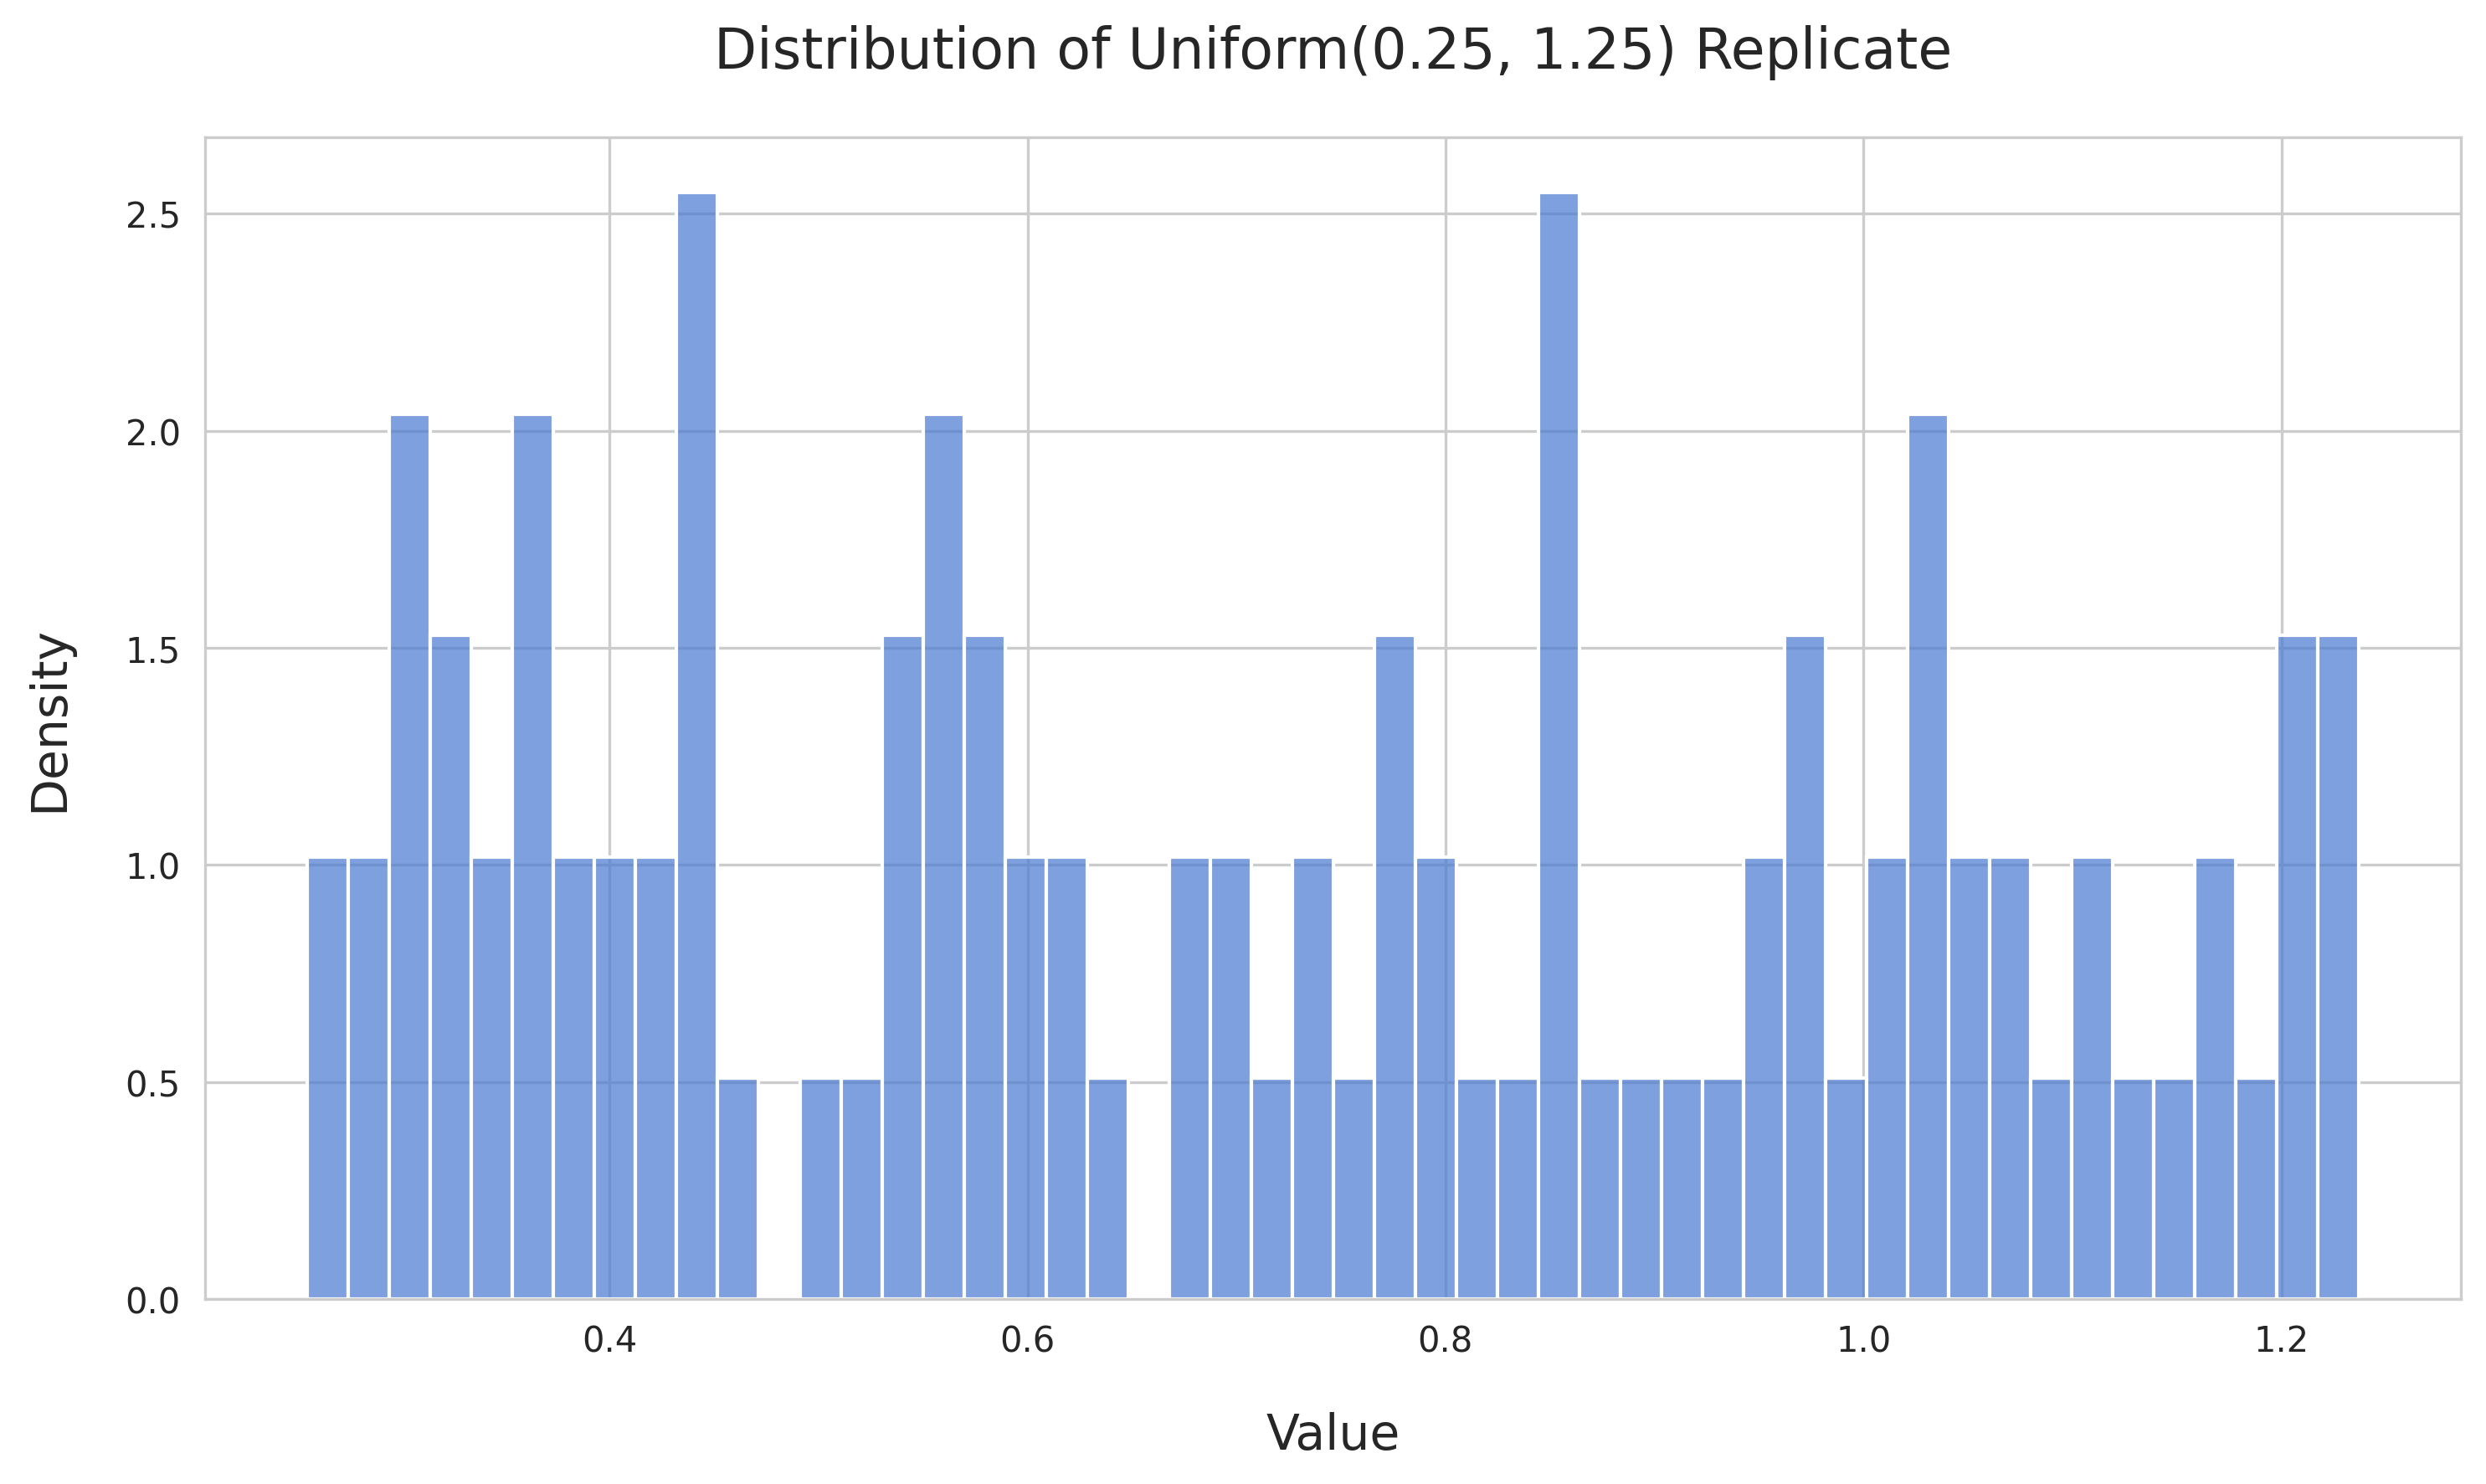
\includegraphics[width=0.95\textwidth]{figures/uniform_replicate.png}
  
  \textbf{Figure 3:} Distribution of a replicate from the Uniform(0.25, 1.25) distribution.
\end{center}

\begin{center}
  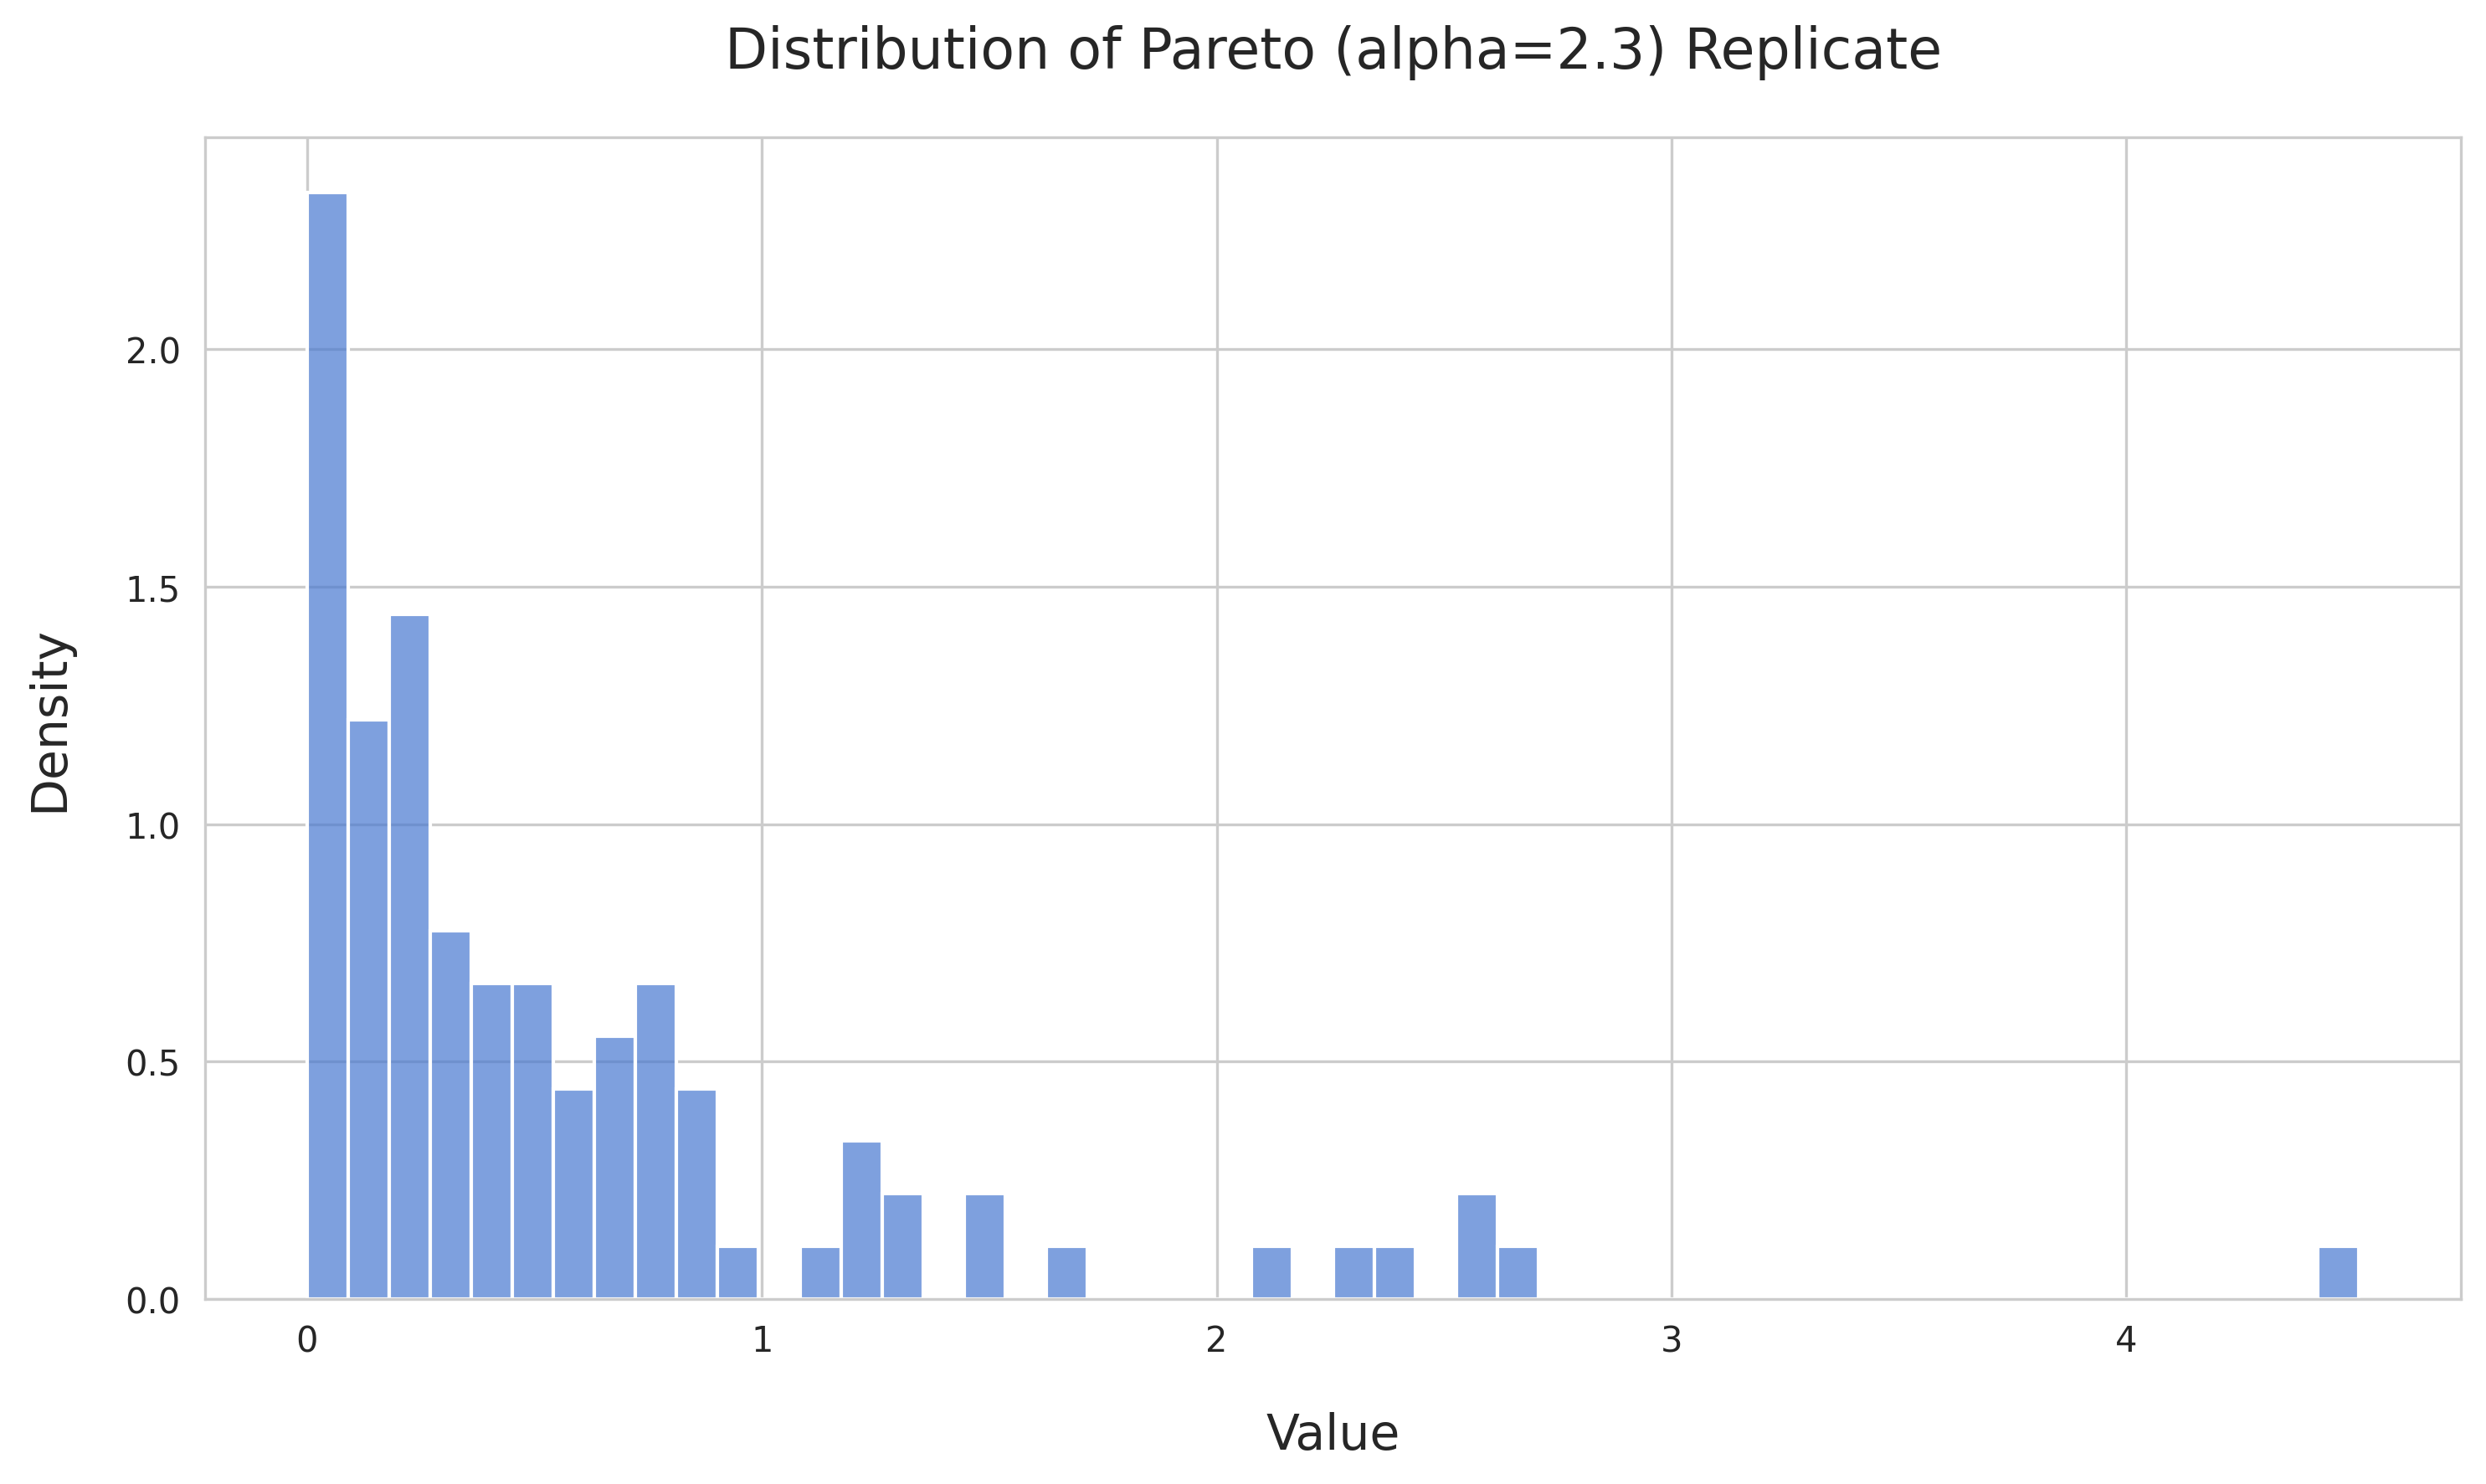
\includegraphics[width=0.95\textwidth]{figures/power_replicate.png}
  
  \textbf{Figure 4:} Distribution of a replicate from the Pareto($ \alpha=2.3$) distribution.\\
\end{center}

The Uniform replicate plot in Figure 3 shows the generally flat distribution of mass that we would expected across the interval, at least as flat as we could reasonably expect from only 100 samples.\\

The Pareto replicate plot in Figure 4 exhibits the characteristic right-skewed shape of a heavy-tailed power-law distribution, like the ones we have discussed in lecture. Most of the distribution mass is concentrated near zero, and a long tail extends out to larger values, showing that generally the probability density decreases with larger values, but extreme values are still present and predictable in the sample.\\

Regarding np.random.power and np.random.pareto, the Canvas announcement made the clarification that we are meant to explore the discrepancy in the distribution shapes these two approaches produce. According to the NumPy documentation, np.random.power draws samples from a power function distribution with positive exponent $a - 1$. The probability density function is:

$$
P(x; a) = a \cdot x^{a-1}, \quad 0 \le x \le 1, \quad a > 0
$$

Also I feel I should mention that the documentation literally states, "The power function distribution is just the inverse of the Pareto distribution". So given that guidance and looking at our case in the assignment, alpha is meant to be set to 3 if using numpy.random.power, making the PDF:

$$
P(x; a) = 3x^2, \quad 0 \le x \le 1
$$

There are definitely a lot of characteristics that distinguish this equation from the power-laws we have looked at in the lecture as well as the one defined by numpy.random.pareto (bounded interval, increasing density instead of decreasing, etc.), but let's look first at the Pareto distribution PDF. np.random.pareto(a) samples from a Pareto Type II distribution with shape parameter $a$ and implicit scale $m=1$, which has the probability density function:

$$
p(x) = \frac{a}{(1+x)^{a+1}}, \quad x \ge 0
$$

Applying our setting of $a=2.3$ gives the PDF $ p(x) = \frac{2.3}{(1+x)^{3.3}}$. So the np.random.power approach is described by $ 3x^2 $ on $ [0,1] $, where the exponent is positive and the function value increases as x approaches 1, concentrating almost all probability mass near the upper bound with no capacity for extreme outliers beyond this range. In contrast, np.random.pareto is described by $ \frac{2.3}{(1+x)^{3.3}} $ on $ [0, \infty) $, where the function value decreases as x increases (since $(1+x)^{3.3}$ in the denominator grows), placing most mass near zero but maintaining enough probability in the tail to produce occasional extreme values.\\

This distribution produced by numpy.random.power seems distinctly different from what we have discussed in lecture. After having applied the settings given in the assignment instructions, the inverse relationship and subsequent effect on the distribution shape was readily obvious, but that still did not explain why numpy.random.power is set up in this manner; it seems inconsistent with what I have come to understand Power-Law to be from class. My understanding from the documentation and community support online has led me to believe that numpy.random.power generates from a power function distribution, with an exponential relationship to its alpha parameter, which is inconsistent with the general power-law relationship that we established in lecture; that is, $ p(x) \propto x^{-a} $. The Pareto Type II distribution from np.random.pareto, on the other hand, exhibits the characteristic heavy-tail behavior where the denominator $(1+x)^{3.3}$ creates the decreasing density function consistent with power-law relationship. They are related but distinctly different in their construction and produce starkly different distribution shapes as a result.

\newpage